\section{Результати алгоритму Б-К та згорткових нейромереж}

В даній роботі добре проявив себе метод Б-К (рис. \ref{fig:bk_examples}),
а саме програмна бібліотека PyMaxflow,
що базується на бібліотеці maxflow, автором якої є сам Володимир Колмогоров.

Переваги алгоритму Б-К:
\begin{enumerate}
    \item алгоритм Б-К досить швидко будує мінімальний розріз. В середньому
          потрібно 0.2 секунди для кадру розміром $330 \times 640$.
    \item даний метод не потребує ніякої передобробки, тобто не потрібно навчати
          як нейронну нейромережу.
\end{enumerate}

Недоліки алгоритму Б-К:
\begin{enumerate}
    \item оскільки даний метод локалізує рух на кадрах відео,
          при русі камери практично все, що в кадрі, стає рухомим об'єктом
          (рис.\ref{fig:bk_bad_mask}).
          Частково дана проблема вирішена на другому кроці алгоритму створення панорами
          (алгоритм \ref{al:panorama_creating_algorithm});
    \item якщо викладач практично не рухається впродовж довгого часу, відповідно не потрапляє
          на маску рухомих об'єктів, він може потрапити на панорамний слайд.
\end{enumerate}
\begin{figure}[H]
    \centering

    \subfloat[\cite{video:krygin_geometry}]{
        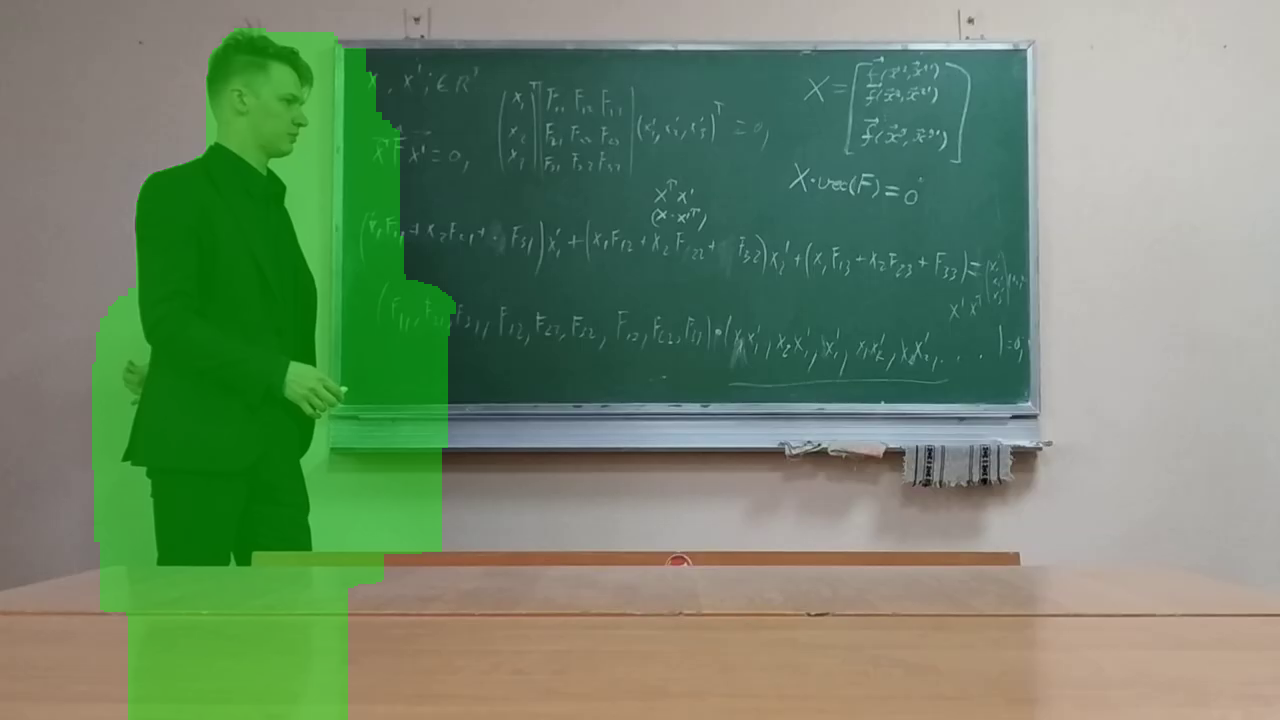
\includegraphics[width=0.35\textwidth]{images/krygin_geometry_bk_17350}
    }
    \subfloat[\cite{video:mmzi:algebra_geometry}]{
        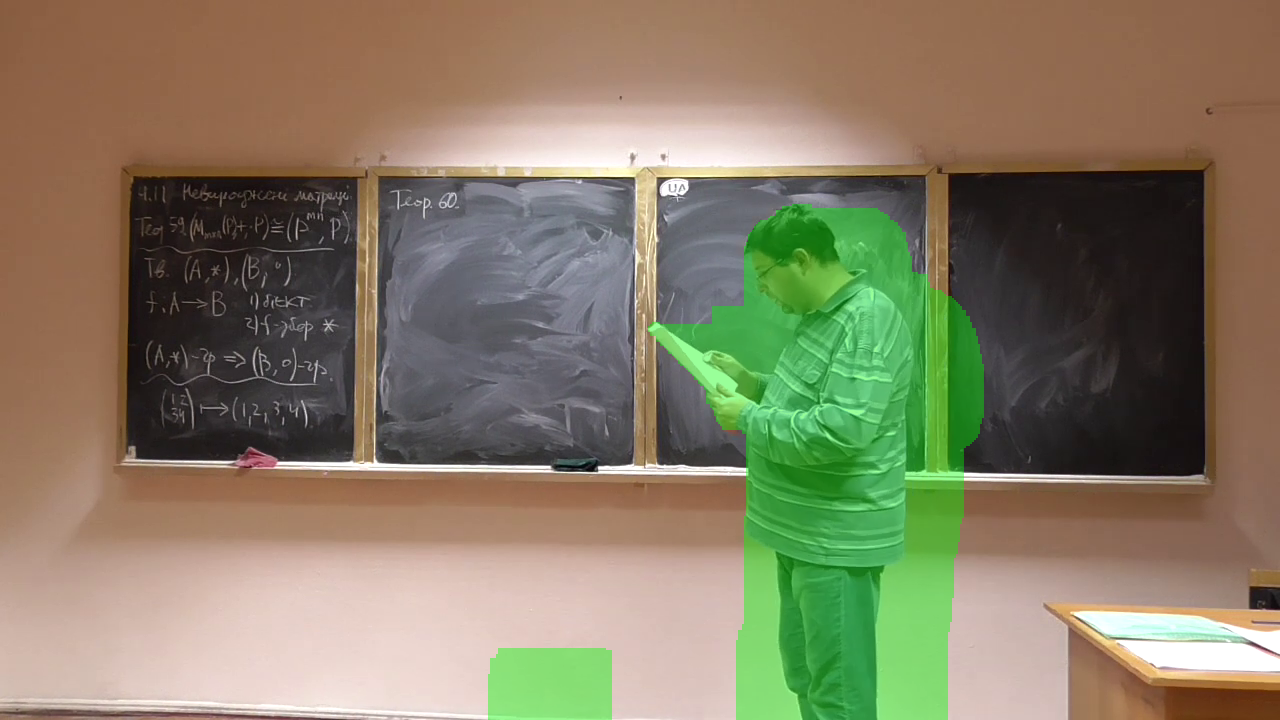
\includegraphics[width=0.35\textwidth]{images/algebra_geometry_bk_9650}
    }\\
    \subfloat[\cite{video:mmzi:yakovlev_numbers_theory}]{
        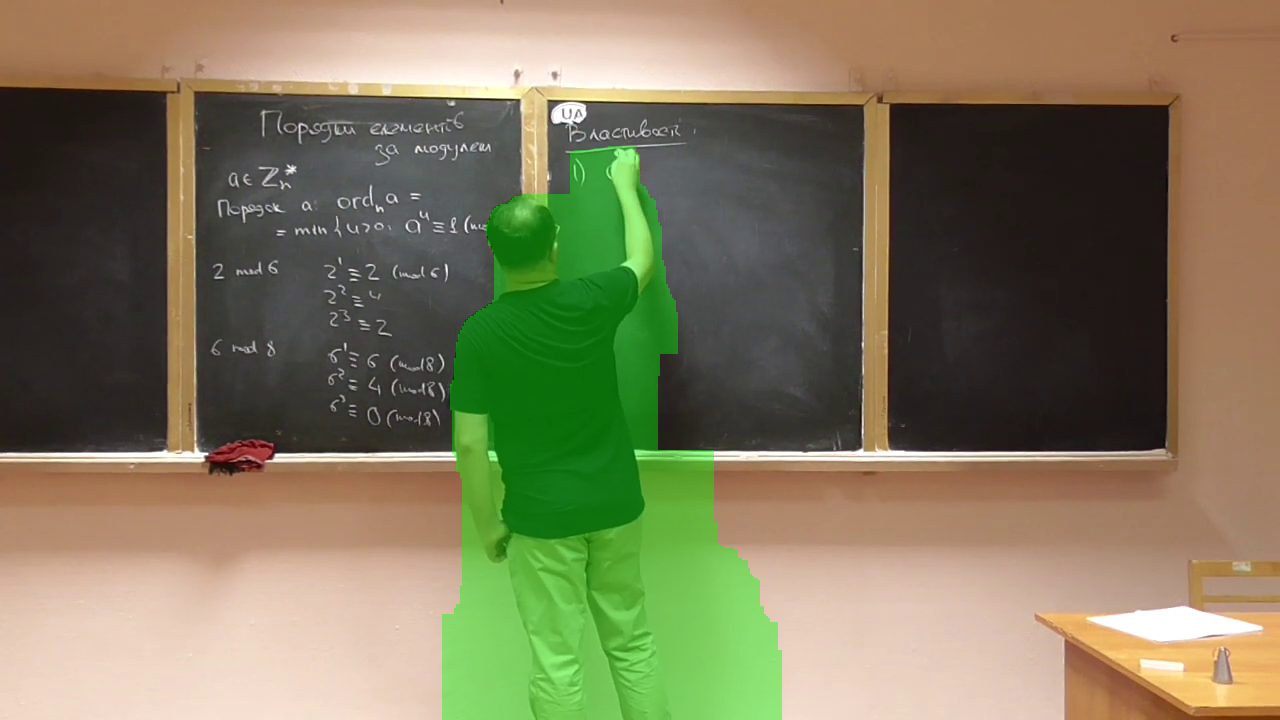
\includegraphics[width=0.35\textwidth]{images/yakovlev2_bk_6500}
    }
    \subfloat[\cite{video:dorohovtsev_wiener_process}]{
        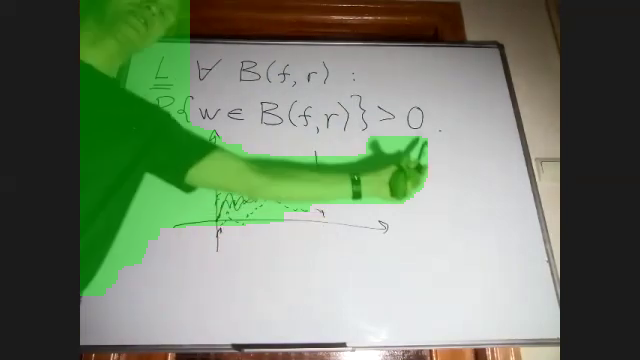
\includegraphics[width=0.35\textwidth]{images/dorohovtsev2_bk_10650}
    }
    \caption{Приклад роботи алгоритму Б-К для отримання маски рухомих об'єктів
        \label{fig:bk_examples}
    }
\end{figure}
\begin{figure}[H]
    \centering

    \subfloat[]{
        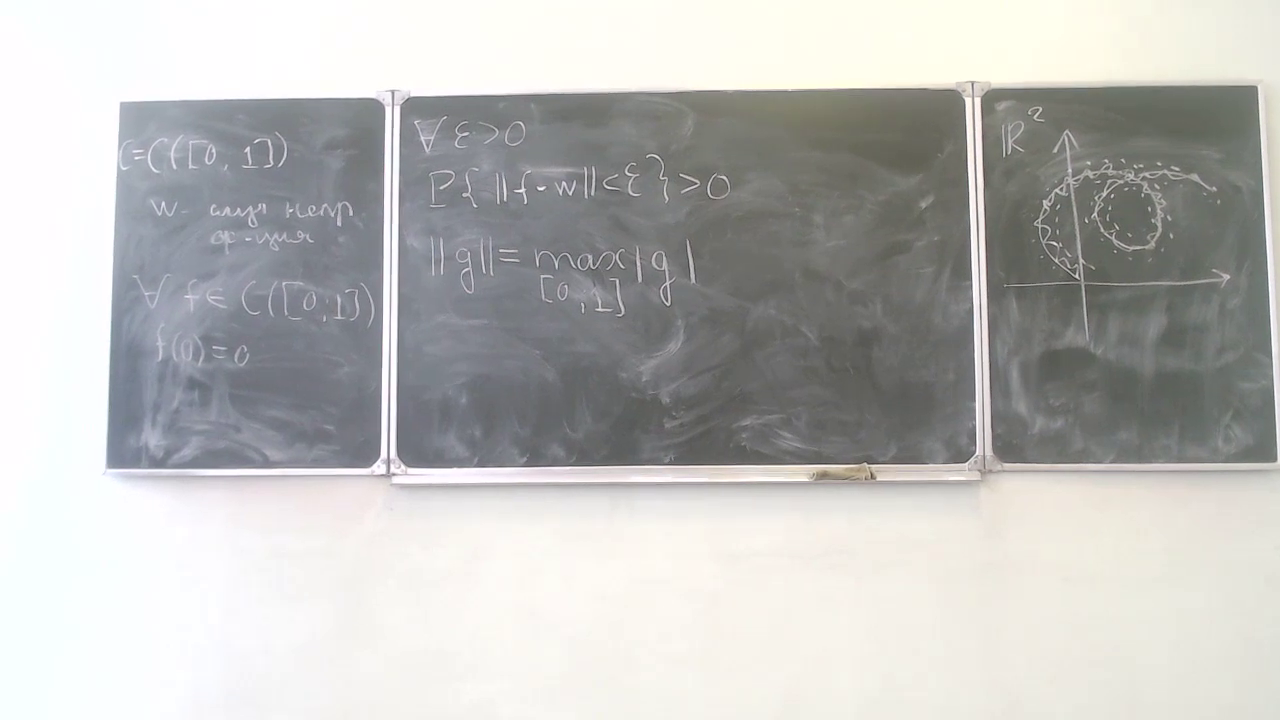
\includegraphics[width=0.35\textwidth]{images/bad_prev_dorohovtsev_bk_5790}
    }
    \subfloat[]{
        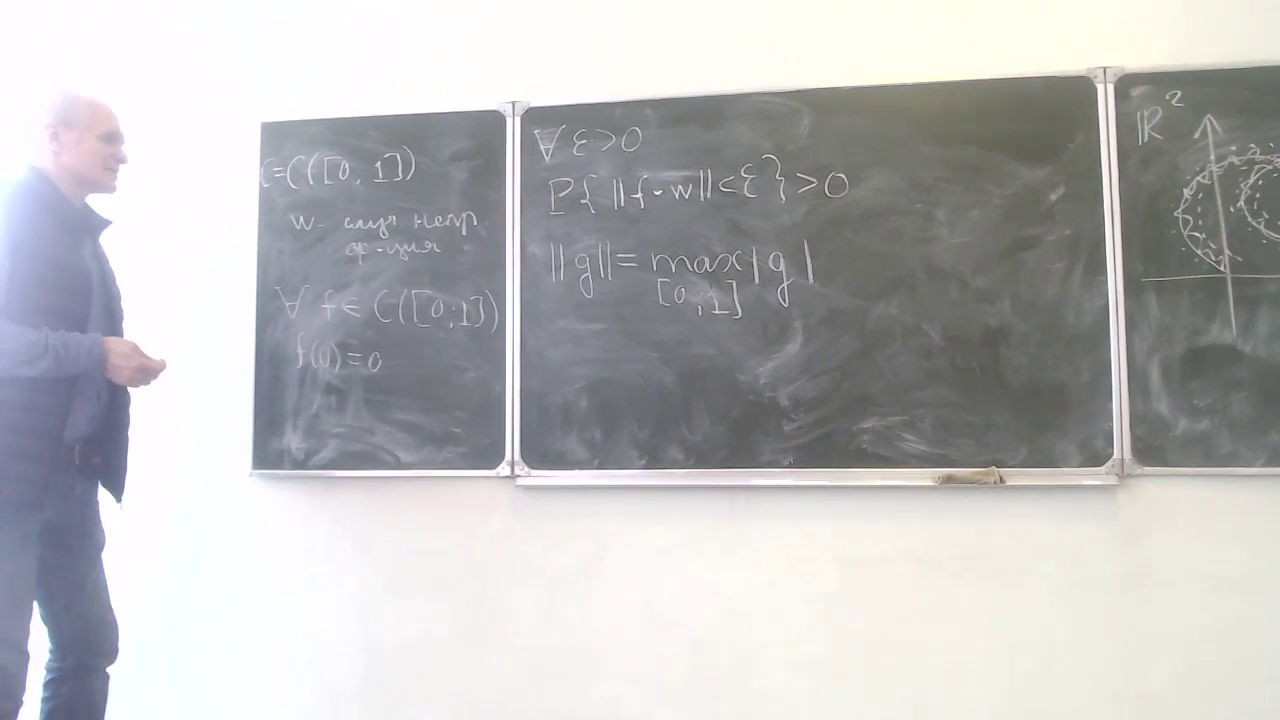
\includegraphics[width=0.35\textwidth]{images/bad_next_dorohovtsev_bk_5840}
    } \\
    \subfloat[]{
        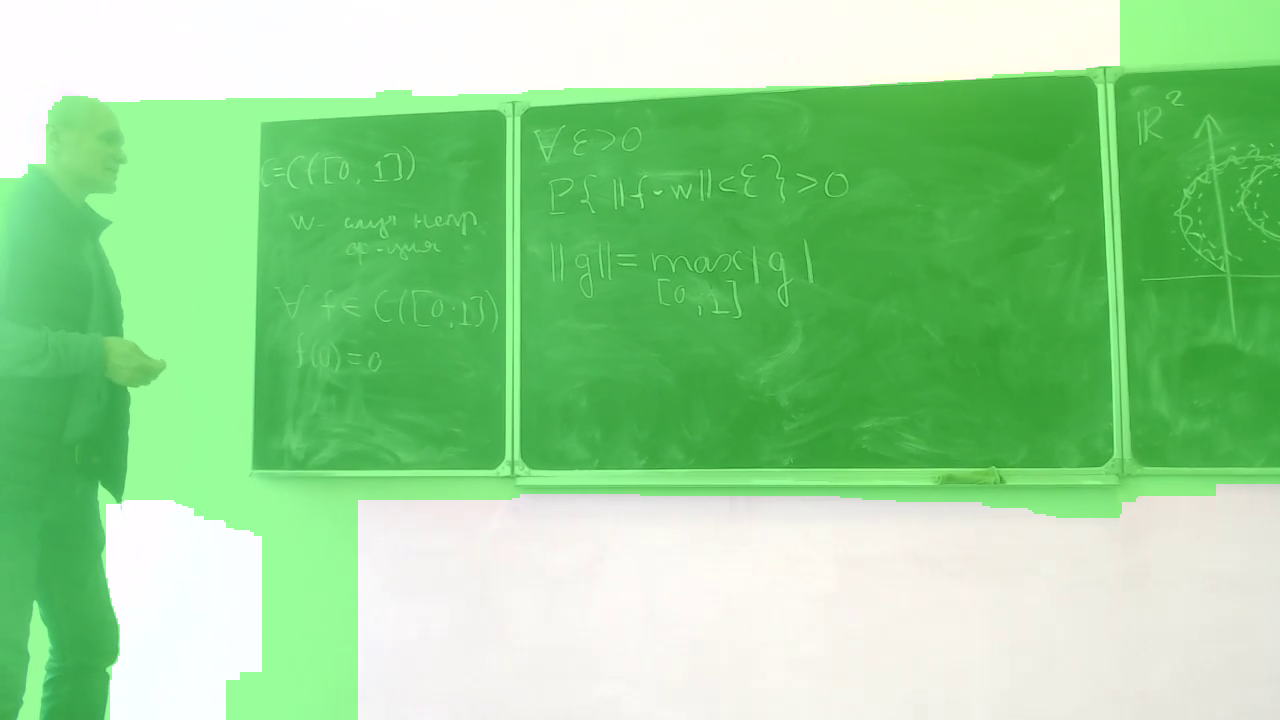
\includegraphics[width=0.35\textwidth]{images/bad_dorohovtsev_bk_example_5840}
    }
    \caption{Приклад поганої маски рухомих об'єктів з відео \cite{video:dorohovtsev_spetskurs_vesna}
        \label{fig:bk_bad_mask}
    }
\end{figure}

\section{Результати застосування згорткових нейромереж}

Переваги використання згорткових нейромереж:
\begin{enumerate}
    \item згорткові нейромережі для детекції людини, що були використані в даній роботі,
          є теж досить швидкими, оскільки були створені для мобільних пристроїв;
    \item детекція людини не залежить від руху камери, тому навіть ті кадри, що
          отримуються під час руху камери, будуть застосовані для створення панорами;
    \item результати експериментів свідчать про високу точність локалізації викладача.
\end{enumerate}

Недоліки використання згорткових нейромереж:
\begin{enumerate}
    \item якщо викладач має в руці якийсь предмет (листок паперу чи маркер), то дані
          об'єкти нейромережа не локалізує, відповідно можуть бути дефекти на панорамі;
    \item розмір програми стає більшим через зберігання ваг.
\end{enumerate}

Значення confidence level $in [0,1]$, що присутнє на прикладах нижче, показує на скільки точно нейромережа
впевнена у детекції людини.

SSDLite320 була використана у даній роботі разом із MobileNetv3, яка слугує в якості нейромережі для
відокремлення ознак  (англ. feature extracting network, backbone). Результати
(рис. \ref{fig:ssdlite320_mobilenet-v3_examples}) свідчать про
непогану точність детекції та швидкість обробки кадру (таб. \ref{tab:speed_methods_table}).

\begin{figure}[H]
    \centering
    \subfloat[\cite{video:krygin_geometry}]{
        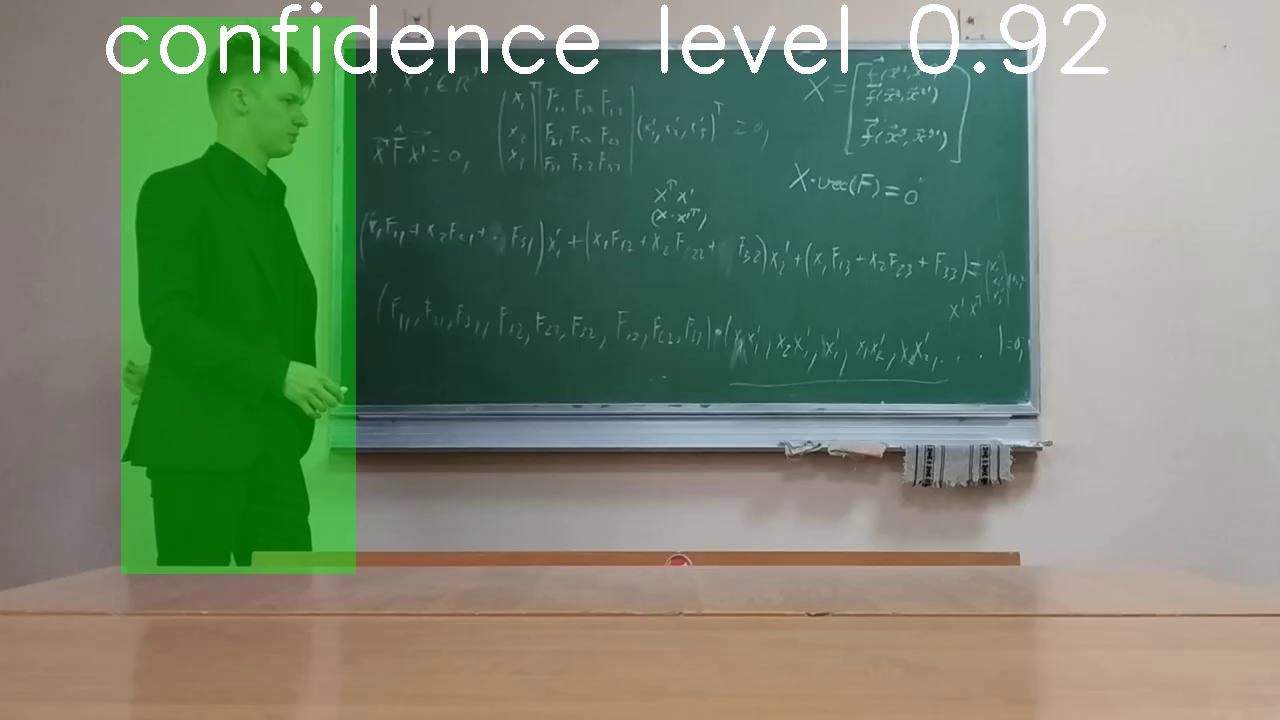
\includegraphics[width=0.35\textwidth]{images/krygin_geometry_ssdlite320_mobilenet_v3_17350}
    }
    \subfloat[\cite{video:mmzi:algebra_geometry}]{
        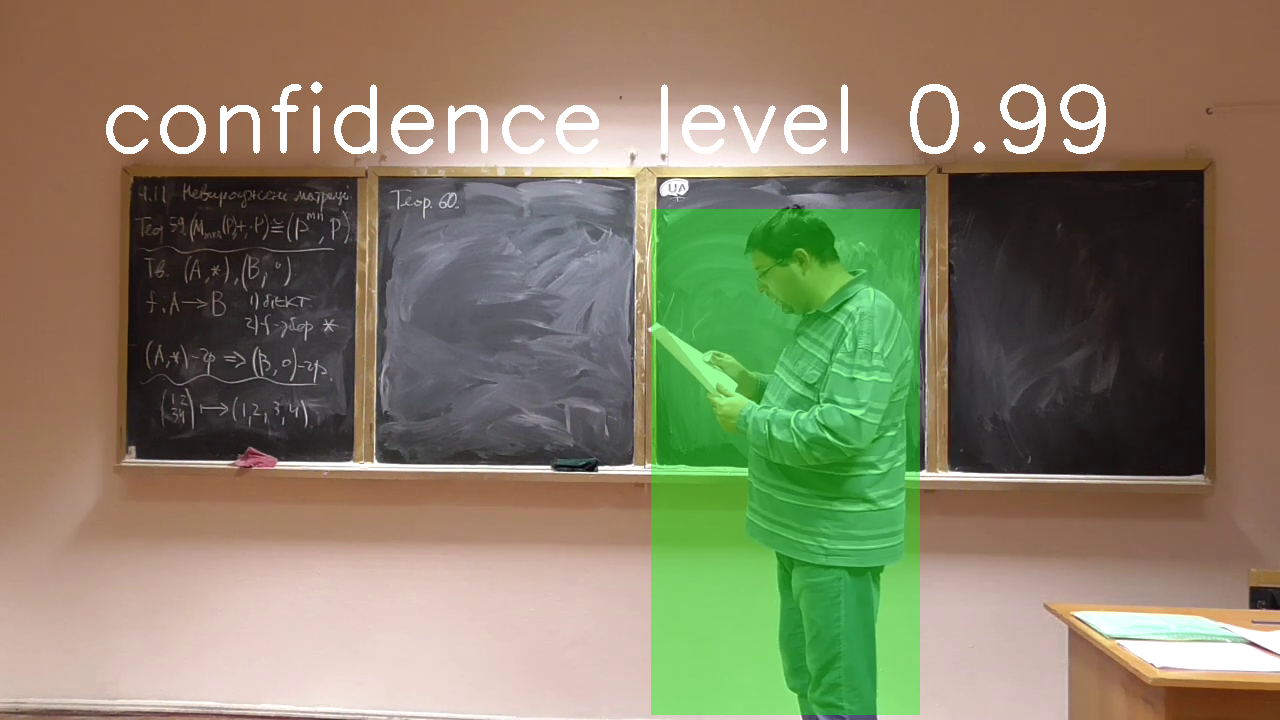
\includegraphics[width=0.35\textwidth]{images/algebra_geometry_ssdlite320_mobilenet_v3_9650}
    } \\
    \subfloat[\cite{video:mmzi:yakovlev_numbers_theory}]{
        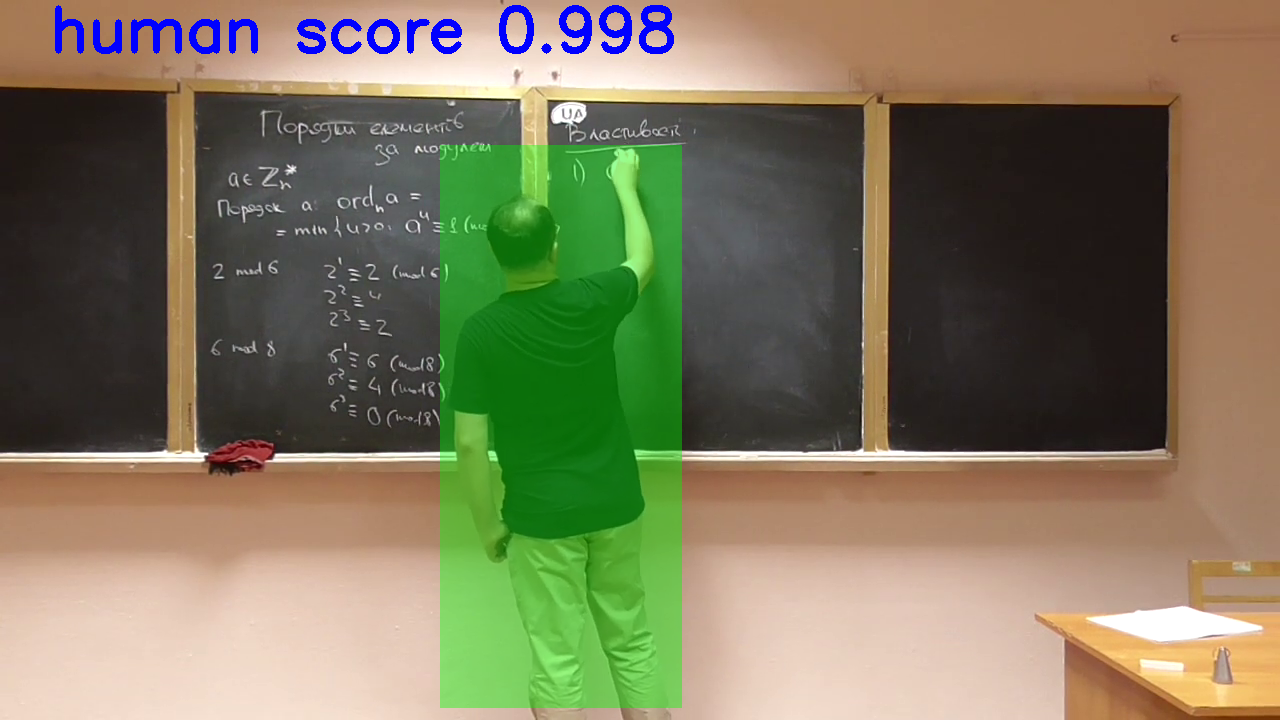
\includegraphics[width=0.35\textwidth]{images/yakovlev2_ssdlite320_mobilenet_v3_6500}
    }
    \subfloat[\cite{video:dorohovtsev_wiener_process}]{
        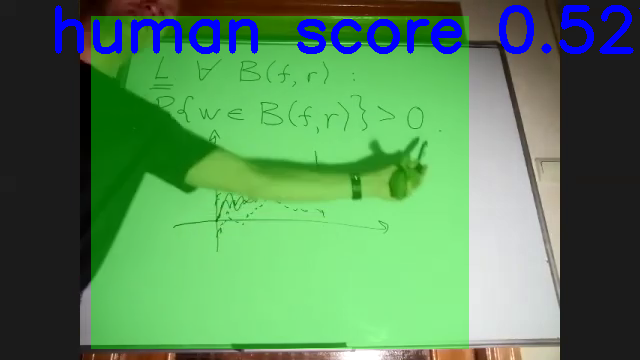
\includegraphics[width=0.35\textwidth]{images/dorohovtsev2_ssdlite320_mobilenet_v3_10650}
    }
    \caption{Приклад роботи ssdlite320-mobilenet-v3
        \label{fig:ssdlite320_mobilenet-v3_examples}
    }
\end{figure}

Так само як і SSDlite320, Faster-RCNN була використана разом з MobileNetv3 в якості backbone нейромережі.
На рис. \ref{fig:fasterrcnn_examples} ми бачимо найвищі значення confidence level. Однак експерименти
показали нестабільність детекції коли викладач частково присутній у кадрі.

\begin{figure}[H]
    \centering
    \subfloat[\cite{video:krygin_geometry}]{
        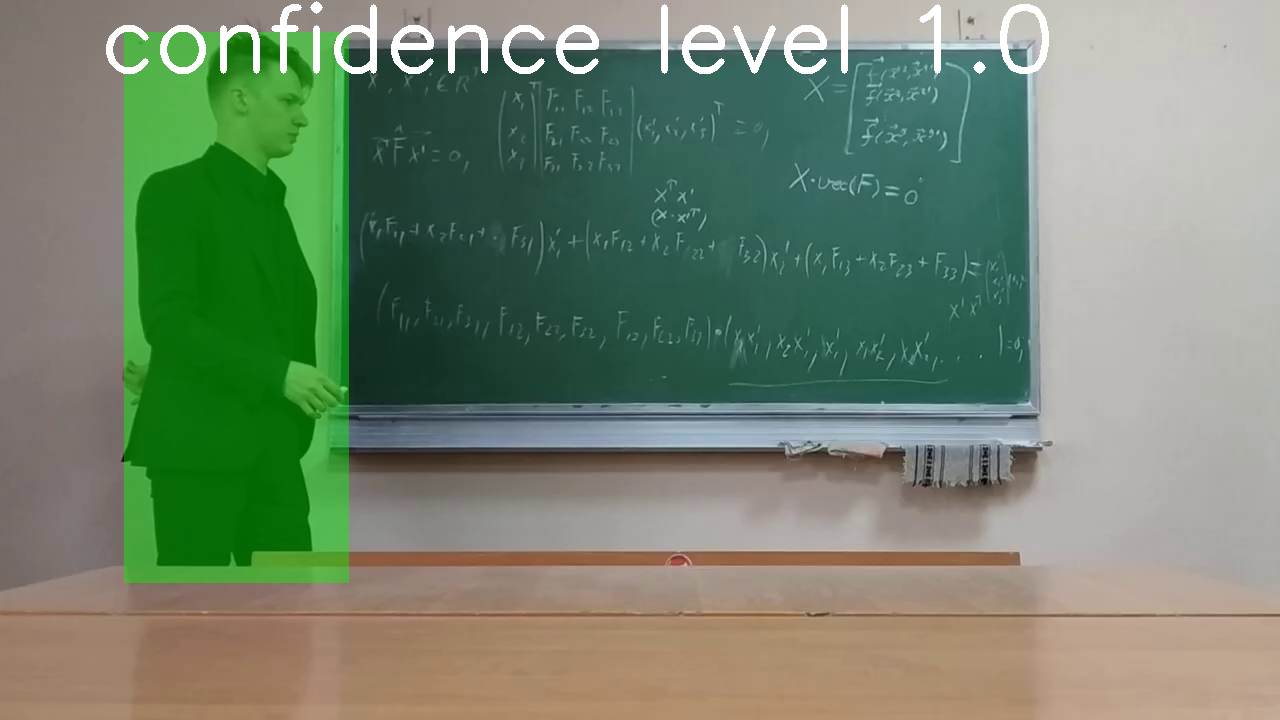
\includegraphics[width=0.35\textwidth]{images/krygin_geometry_fasterrcnn_mobilenet_v3_17350}
    }
    \subfloat[\cite{video:mmzi:algebra_geometry}]{
        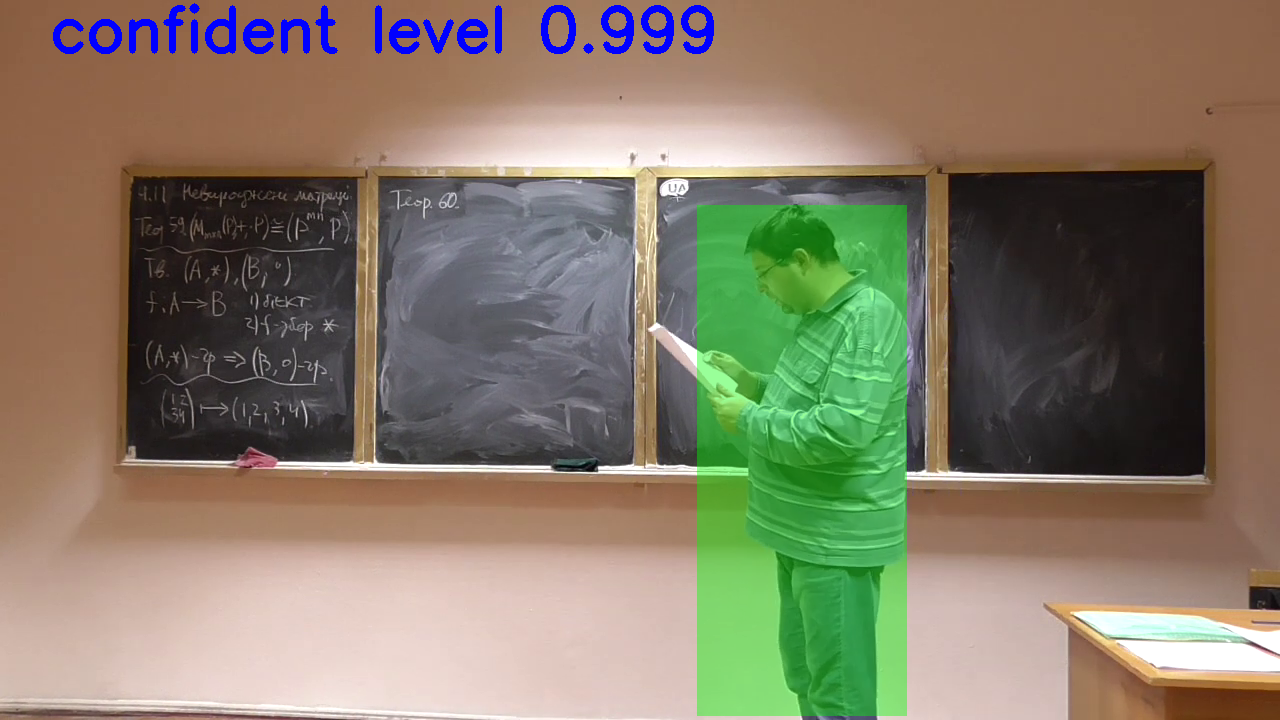
\includegraphics[width=0.35\textwidth]{images/algebra_geometry_fasterrcnn_mobilenet_v3_9650}
    }\\
    \subfloat[\cite{video:mmzi:yakovlev_numbers_theory}]{
        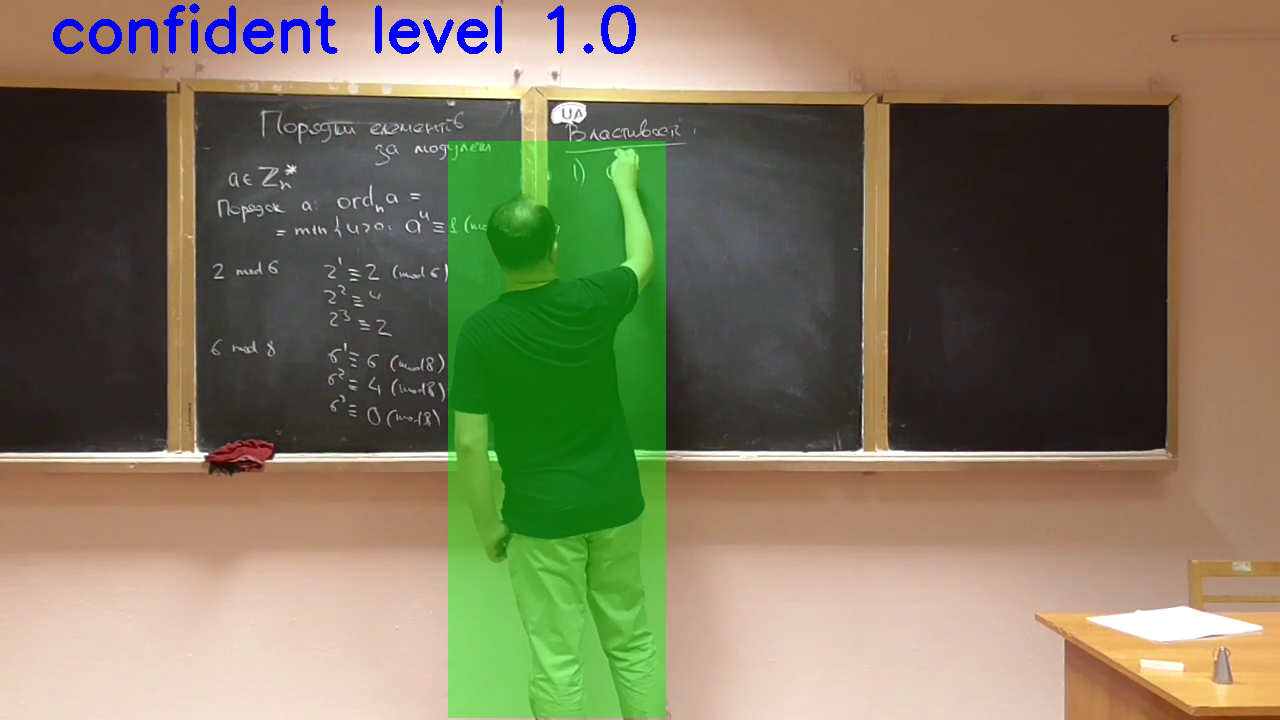
\includegraphics[width=0.35\textwidth]{images/yakovlev2_fasterrcnn_mobilenet_v3_6500}
    }
    \subfloat[\cite{video:dorohovtsev_wiener_process}]{
        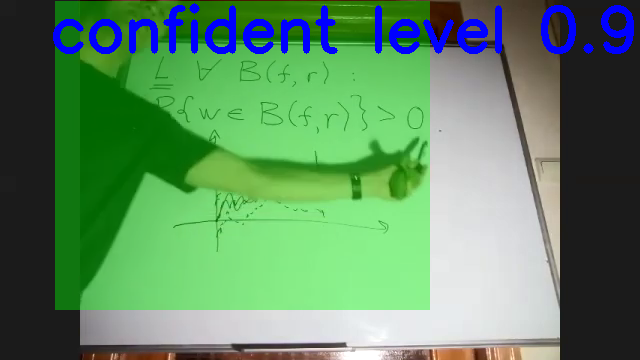
\includegraphics[width=0.35\textwidth]{images/dorohovtsev2_fasterrcnn_mobilenet_v3_10650}
    }
    \caption{Приклад роботи fasterrcnn-mobilenet-v3
        \label{fig:fasterrcnn_examples}
    }
\end{figure}

Найбільш оптимальним методом для прибирання викладача була обрана нейромережа Yolov5n, оскільки вона
дає маску викладача навіть коли він частково присутній в кадрі, тим самим зменшує ймовірність появи
дефектів на панорамі. Результати (рис. \ref{fig:yolov5n_examples}) свідчать про високу точність детекції
людини.

\begin{figure}[H]
    \centering
    % yolov5n
    \subfloat[\cite{video:krygin_geometry}]{
        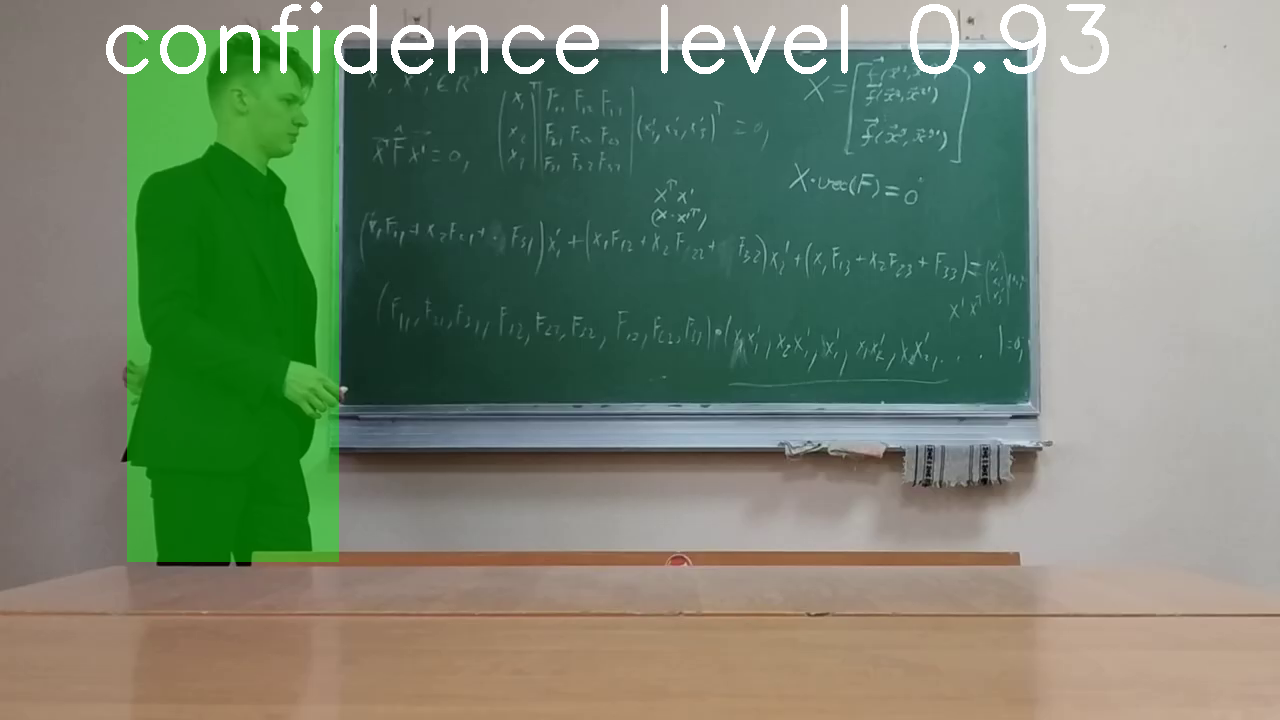
\includegraphics[width=0.35\textwidth]{images/krygin_geometry_yolov5n_17350}
    }
    \subfloat[\cite{video:mmzi:algebra_geometry}]{
        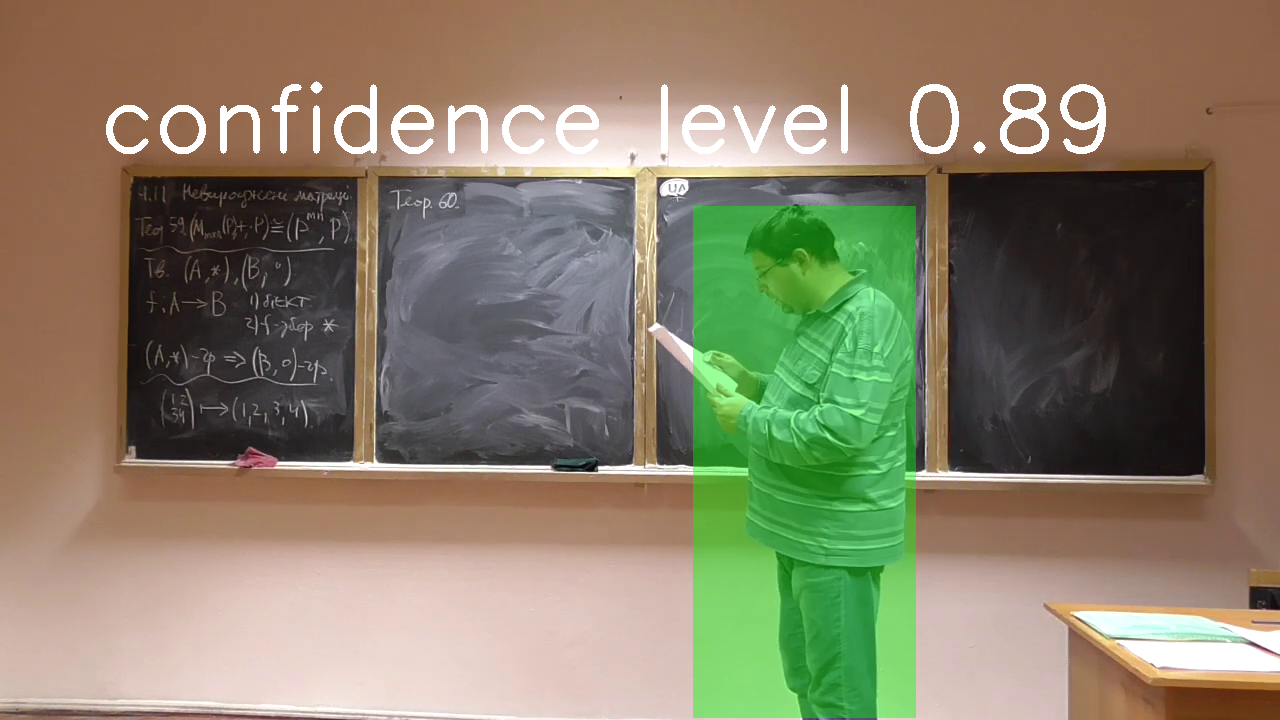
\includegraphics[width=0.35\textwidth]{images/algebra_geometry_yolov5n_9650}
    } \\
    \subfloat[\cite{video:mmzi:yakovlev_numbers_theory}]{
        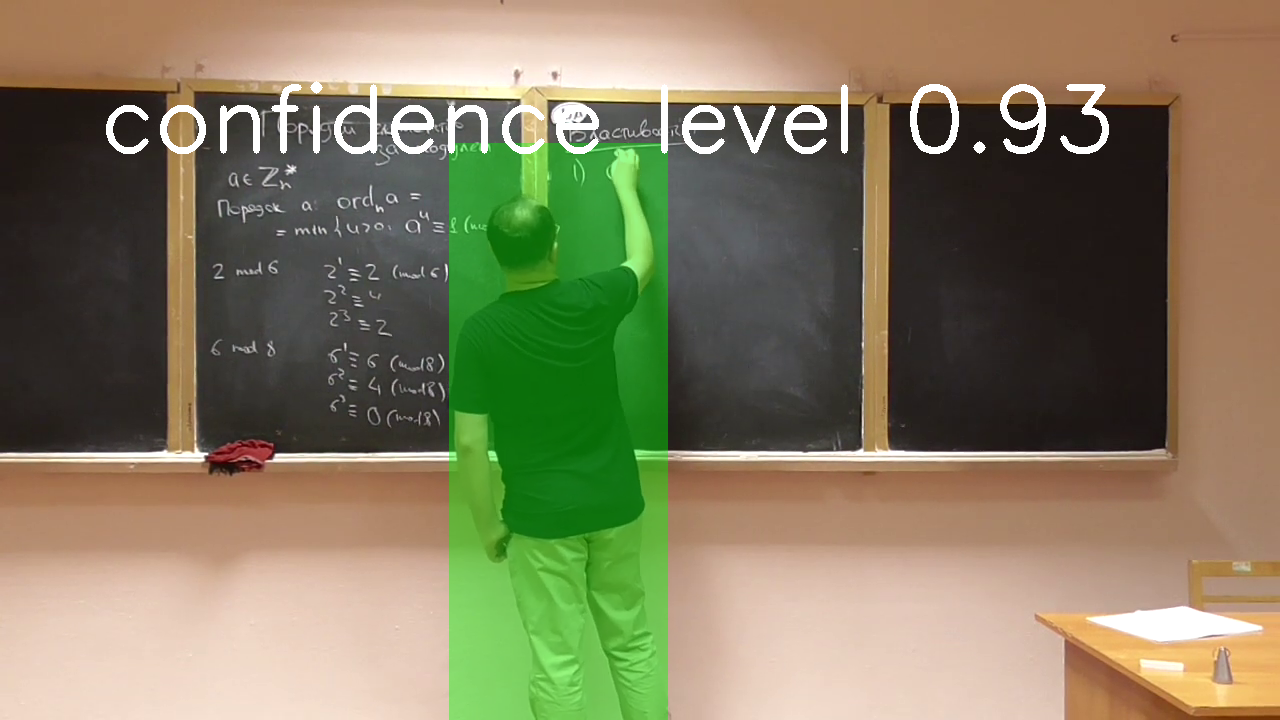
\includegraphics[width=0.35\textwidth]{images/yakovlev2_yolov5n_6500}
    }
    \subfloat[\cite{video:dorohovtsev_wiener_process}]{
        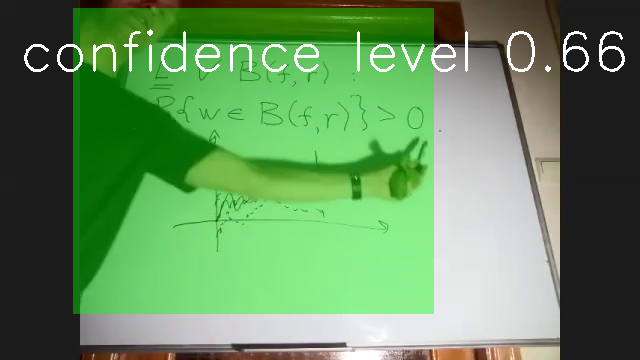
\includegraphics[width=0.35\textwidth]{images/dorohovtsev2_yolov5n_10650}
    }
    \caption{Приклад роботи Yolov5n
        \label{fig:yolov5n_examples}
    }
\end{figure}

\section{Швидкість методів локалізації людини чи рухомих об'єктів}

Було протестовано 1000 разів отримання маски різними методами на картинці $720 \times 1280$ та
отриманий середній час обробки кадру (таб. \ref{tab:speed_methods_table}).
Варто відмітити, що картинка перед входом в шари згорток у згорткових нейромережах зменшується
до базового розміру для входу нейромережі. Така ж компресія робиться і для входу
в алгоритм Б-К, картинка зменшується удвічі.

\begin{table}[H]
    \begin{center}
        \caption{Таблиця швидкості згорткових нейромереж та алгоритму Б-К}
        \label{tab:speed_methods_table}
        \begin{tabular}{|p{1.2in} | p{1.2in} | p{1.2in} | p{1.2in}|}
            \hline
            \textbf{yolov5n} & \textbf{ssdlite320-mobilenet-v3} & \textbf{fasterrcnn-mobilenet-v3} & \textbf{Boykov-Kolmogorov} \\
            \hline
            0.12             & 0.06                             & 0.12                             & 0.22                       \\
            \hline
        \end{tabular}
    \end{center}
\end{table}



Як бачимо з табл. \ref{tab:speed_methods_table}, найшвидшим методом є SSDLite320-mobilenet-v3,
а найдовшим є алгоритм Бойкова-Колмогорова.
Проте емпіричним шляхом було визначено, що кращі результати надає Yolov5n.

\section{Результати створення панорами}

У створенні панорами існує чимало нюансів, оскільки результат буде сильно
залежати від вхідних параметрів, що надасть користувач інформаційної технології.
Наприклад у випадку використання алгоритму Бойкова-Колмогорова, як методу що допомагає
прибрати викладача з відео потрібно надати значення ваг між ребрами. Якщо використати
нейронні мережі, то тут важливо вказати мінімальний рівень confidence level, по якому нейромережа
буде детектувати людину чи ні.

Як ми бачимо на прикладах (рис. \ref{fig:panorama:example_2}, \ref{fig:panorama:example_3}) панорами
вийшли досить якісними. Тут видно, що в майбутньому потрібно детектувати дошку, оскільки поза нею
залишаються непотрібні об'єкти. До того ж, якщо ці об'єкти не є плоскими як дошка, то
матриця гомографії не буде достатньо точною, а це вже вплине на панорамну склейку.

\begin{figure}[H]
    \centering
    \subfloat[Панорама з відео \cite{video:mfti:kombinatorika}]{
        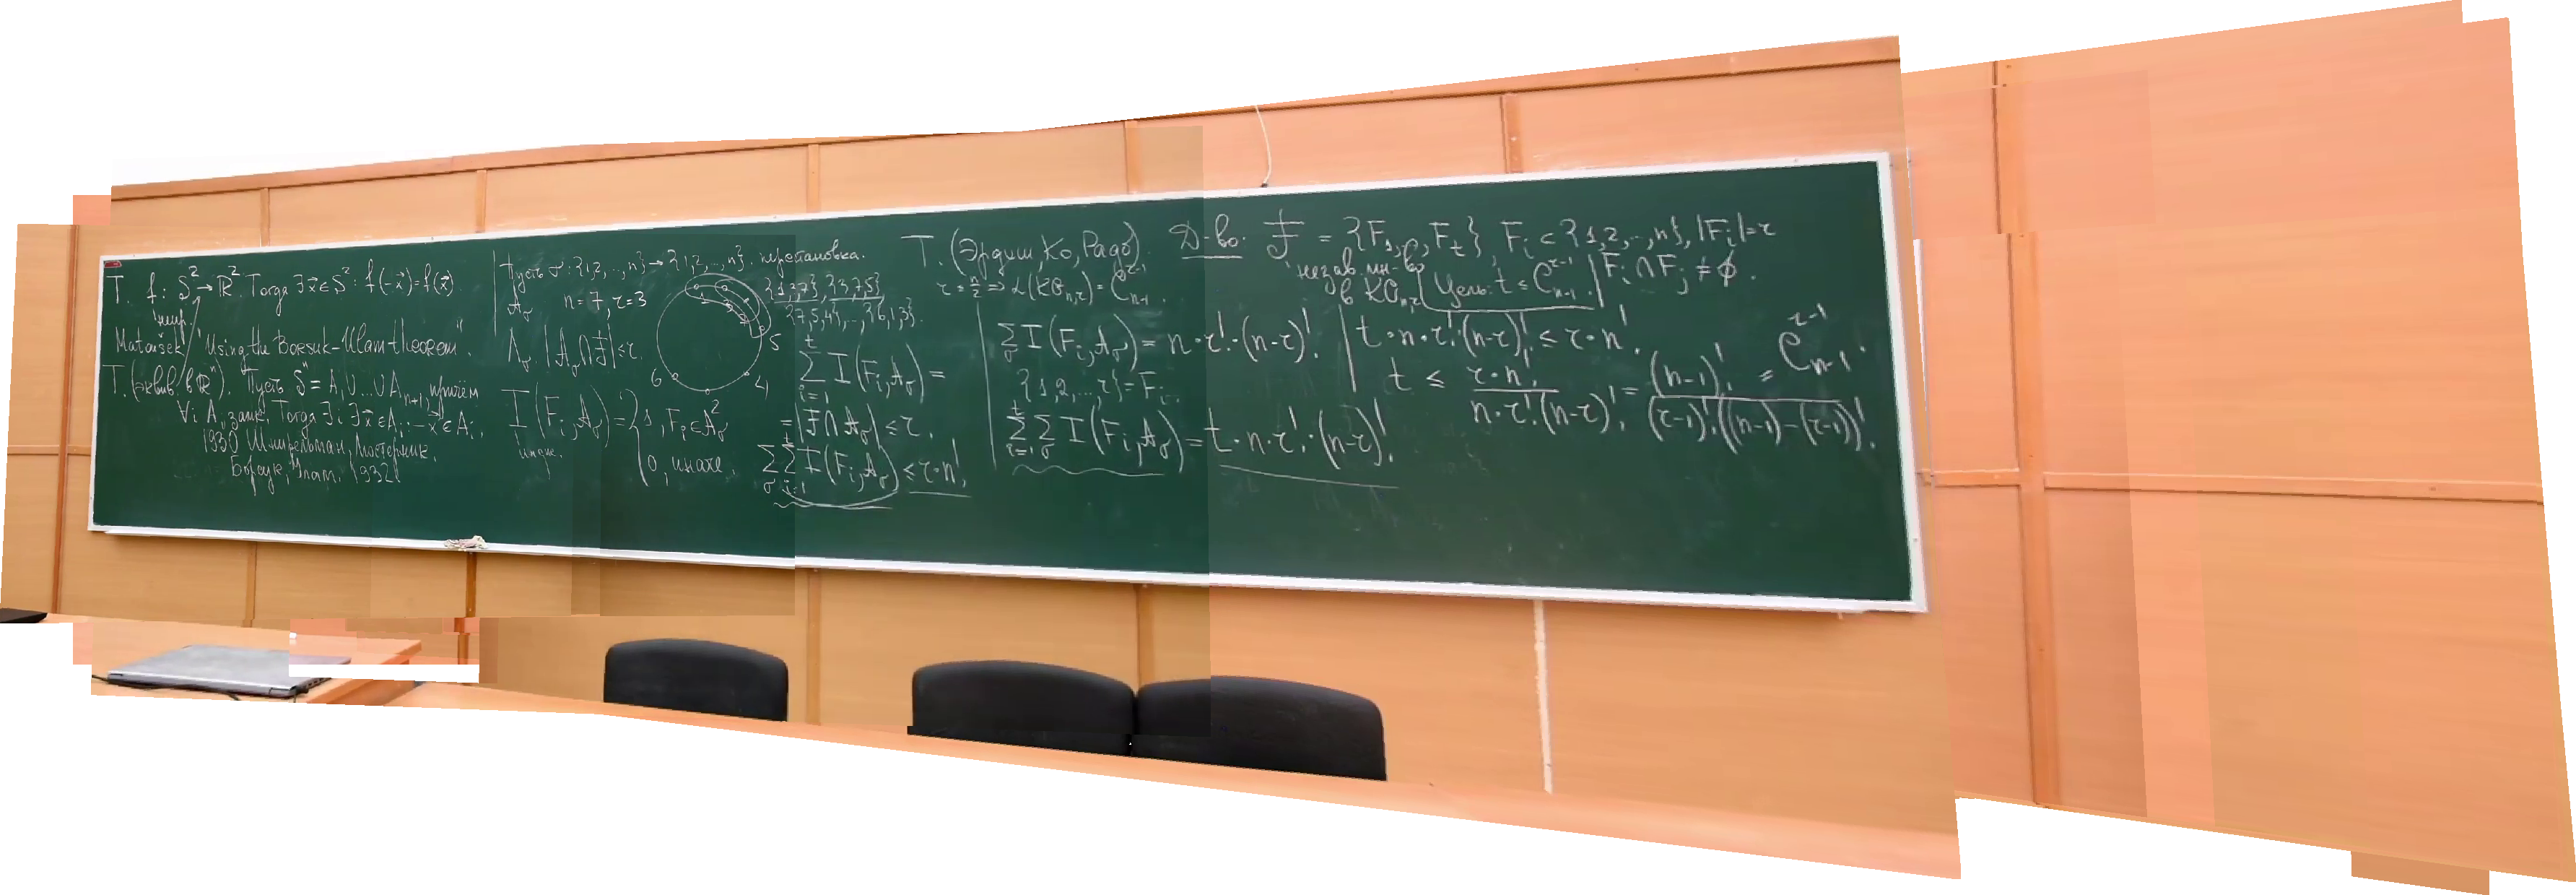
\includegraphics[width=0.7\textwidth]{images/panorama_example_2}
        \label{fig:panorama:example_2}
    }\\
    \subfloat[Панорама з відео \cite{video:mfti:algebra_structure}]{
        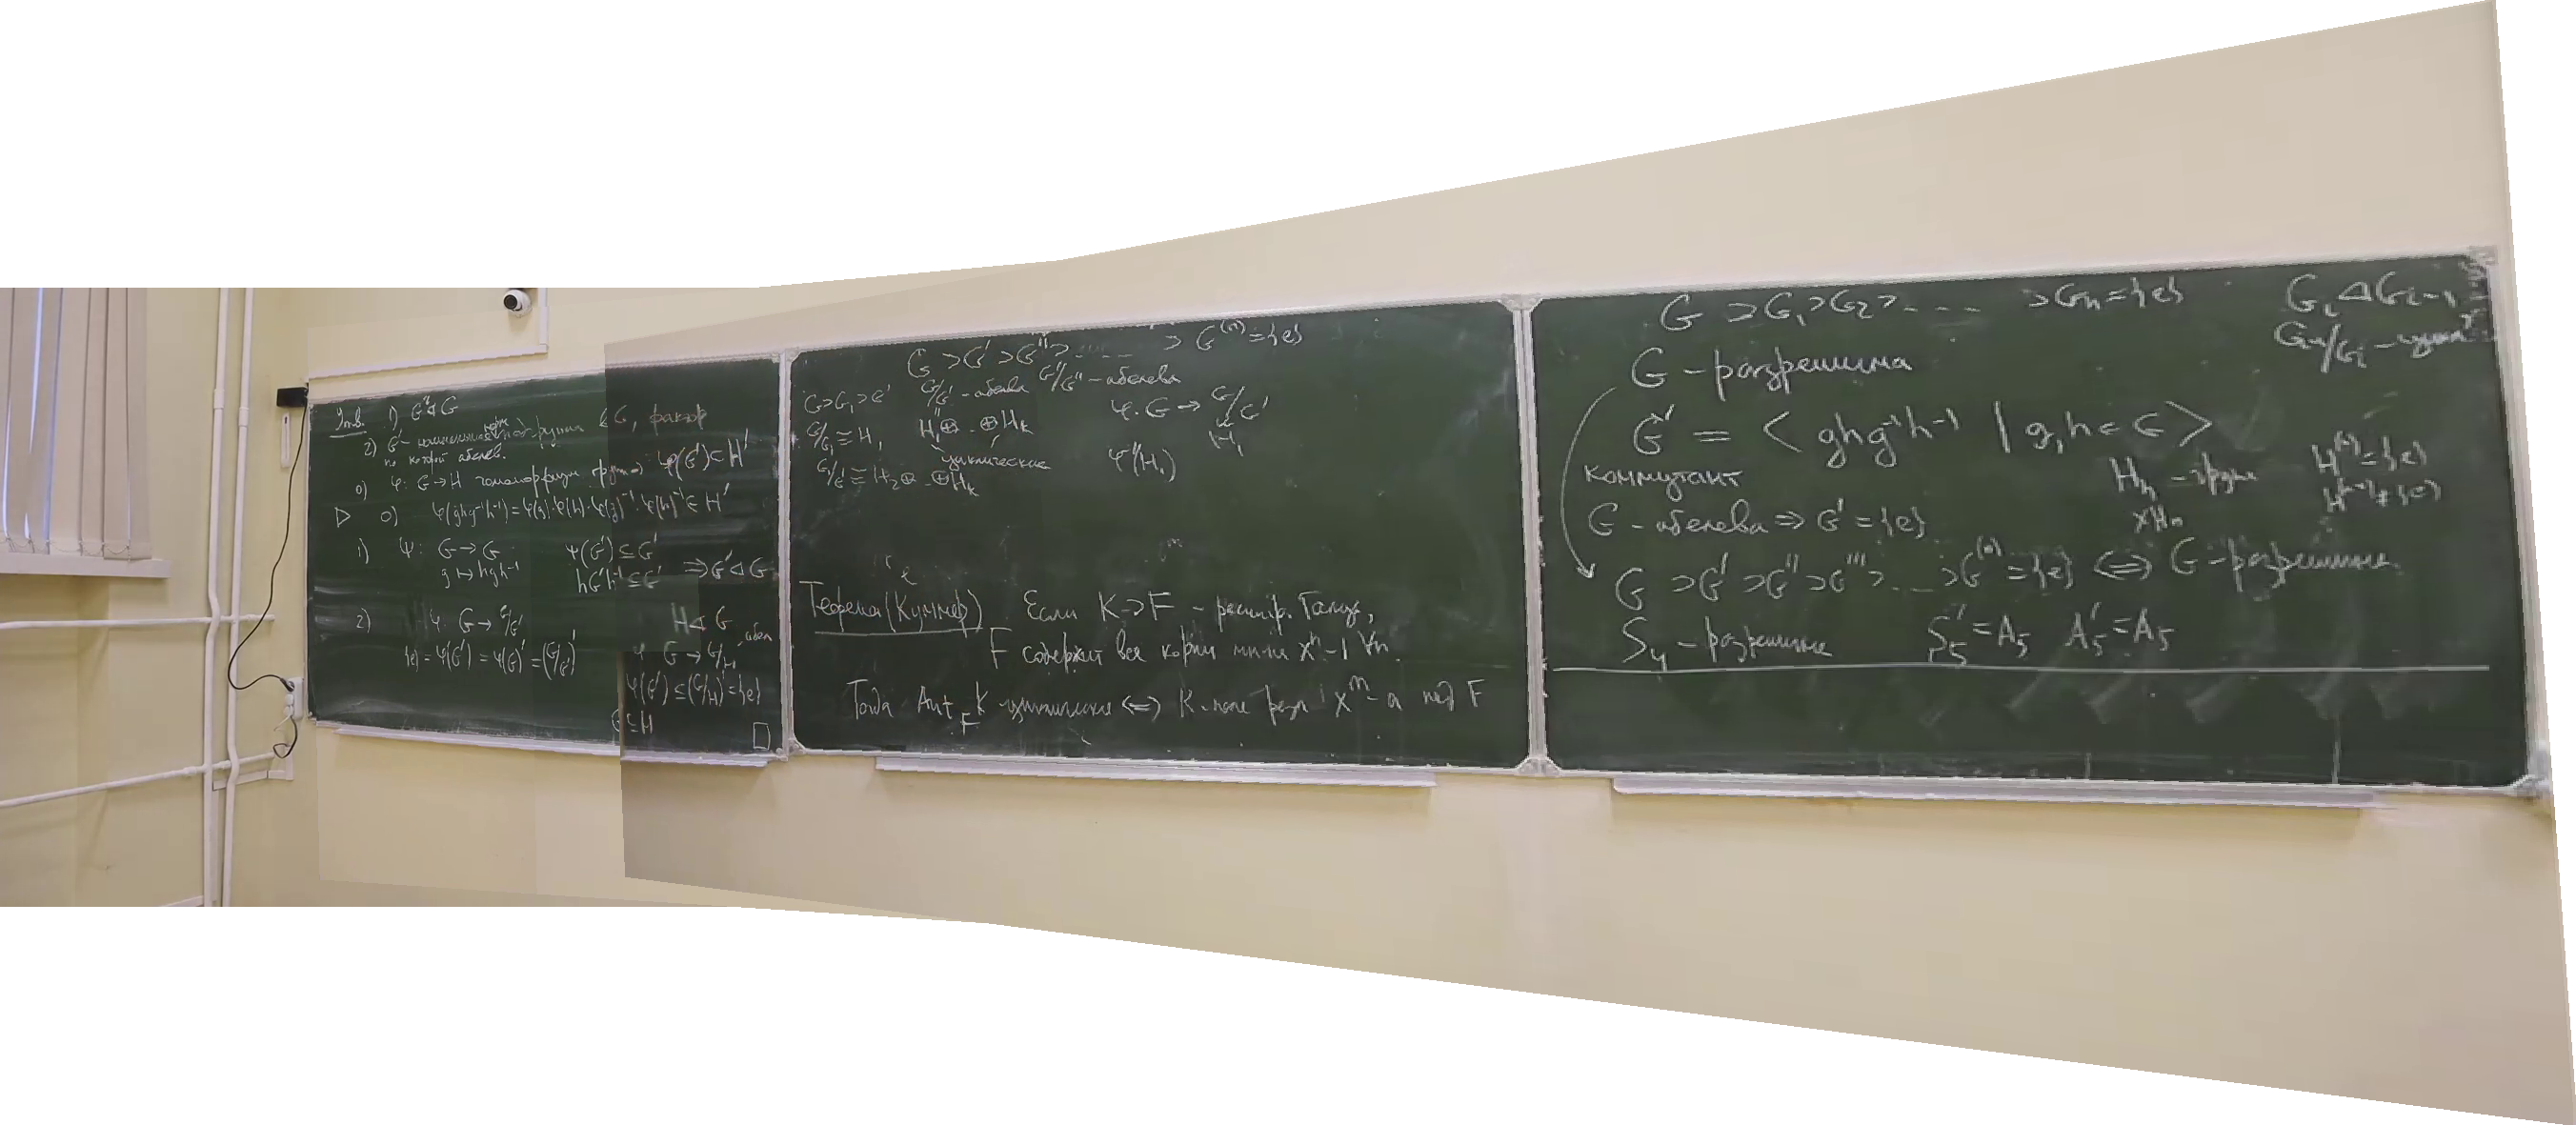
\includegraphics[width=0.7\textwidth]{images/panorama_example_3}
        \label{fig:panorama:example_3}
    }
    \caption{Приклади панорами отриманої без викладача
    }
\end{figure}

Як можна побачити на рис. \ref{fig:panorama_stats_graph}, швидкість створення панорами сильно залежить
від її розміру, тому це і доводить причину детектингу дошки.

\begin{figure}[H]
    \centering
    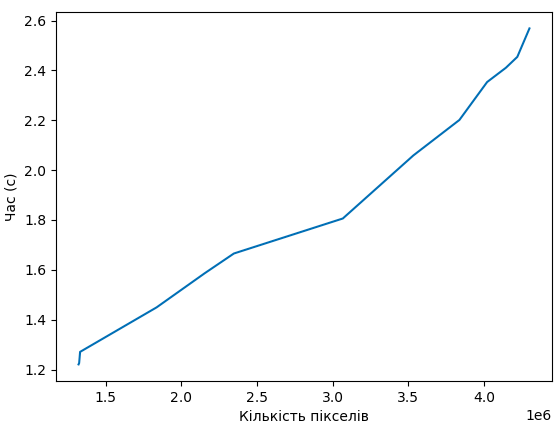
\includegraphics[width=0.45\textwidth]{images/panorama_stats_graph}
    \caption{Графік залежності швидкості однієї ітерації створення панорами
        від кількості пікселів на ній для відео \cite{video:mfti:kombinatorika}
        \label{fig:panorama_stats_graph}
    }
\end{figure}

\section{Результати використання швидкої медіани}

На рис. \ref{fig:median:after_denoising} можна побачити як медіана справляється з шумом
та артефактами компресії.  Написи стали більш чіткими, а фон дошки більш однорідним.
Даний алгоритм доданий до інформаційної технології перетворення відео з дошки у слайди.

\begin{figure}[H]
    \centering
    \subfloat[До]{
        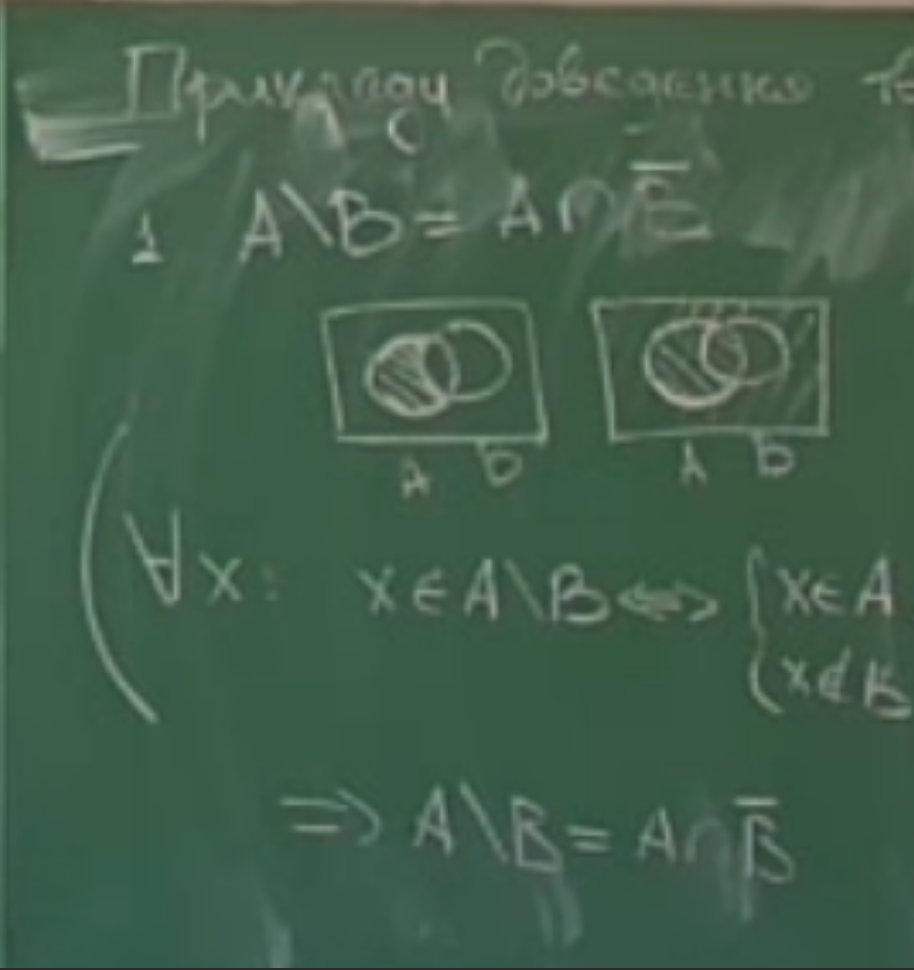
\includegraphics[width=0.35\textwidth]{images/frame_before_median}
    }
    \subfloat[Після]{
        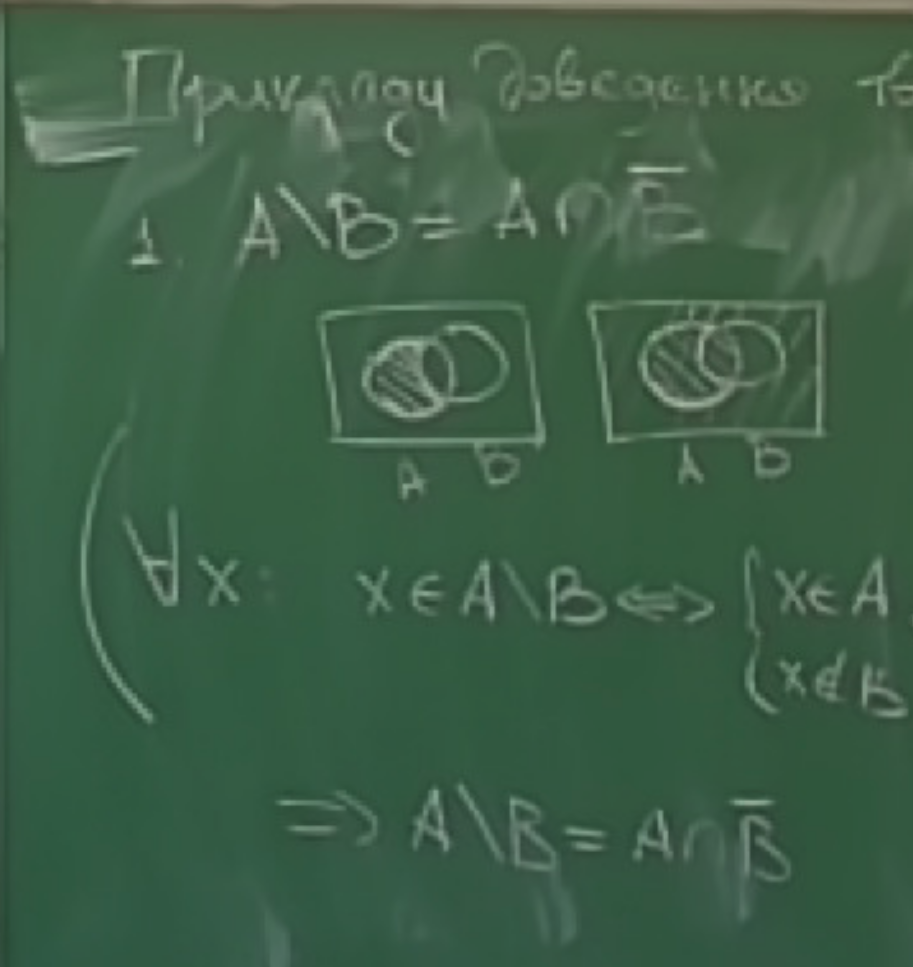
\includegraphics[width=0.35\textwidth]{images/frame_after_median}
        \label{fig:median:after_denoising}
    }
    \caption{Приклад роботи медіани для зображень \cite{video:mmzi:yakovlev_discrete_math}
    }
\end{figure}
